% (find-LATEX "2022-2-C3-VR.tex")
% (defun c () (interactive) (find-LATEXsh "lualatex -record 2022-2-C3-VR.tex" :end))
% (defun C () (interactive) (find-LATEXsh "lualatex 2022-2-C3-VR.tex" "Success!!!"))
% (defun D () (interactive) (find-pdf-page      "~/LATEX/2022-2-C3-VR.pdf"))
% (defun d () (interactive) (find-pdftools-page "~/LATEX/2022-2-C3-VR.pdf"))
% (defun e () (interactive) (find-LATEX "2022-2-C3-VR.tex"))
% (defun o () (interactive) (find-LATEX "2022-2-C3-P2.tex"))
% (defun u () (interactive) (find-latex-upload-links "2022-2-C3-VR"))
% (defun v () (interactive) (find-2a '(e) '(d)))
% (defun d0 () (interactive) (find-ebuffer "2022-2-C3-VR.pdf"))
% (defun cv () (interactive) (C) (ee-kill-this-buffer) (v) (g))
%          (code-eec-LATEX "2022-2-C3-VR")
% (find-pdf-page   "~/LATEX/2022-2-C3-VR.pdf")
% (find-sh0 "cp -v  ~/LATEX/2022-2-C3-VR.pdf /tmp/")
% (find-sh0 "cp -v  ~/LATEX/2022-2-C3-VR.pdf /tmp/pen/")
%     (find-xournalpp "/tmp/2022-2-C3-VR.pdf")
%   file:///home/edrx/LATEX/2022-2-C3-VR.pdf
%               file:///tmp/2022-2-C3-VR.pdf
%           file:///tmp/pen/2022-2-C3-VR.pdf
% http://angg.twu.net/LATEX/2022-2-C3-VR.pdf
% (find-LATEX "2019.mk")
% (find-sh0 "cd ~/LUA/; cp -v Pict2e1.lua Pict2e1-1.lua Piecewise1.lua ~/LATEX/")
% (find-sh0 "cd ~/LUA/; cp -v Pict2e1.lua Pict2e1-1.lua Pict3D1.lua ~/LATEX/")
% (find-sh0 "cd ~/LUA/; cp -v C2Subst1.lua C2Formulas1.lua ~/LATEX/")
% (find-CN-aula-links "2022-2-C3-VR" "3" "c3m222vr" "c3vr")

% «.defs»		(to "defs")
% «.defs-T-and-B»	(to "defs-T-and-B")
% «.title»		(to "title")
% «.links»		(to "links")
% «.questao-1»		(to "questao-1")
%
% «.djvuize»		(to "djvuize")



% <videos>
% Video (not yet):
% (find-ssr-links     "c3m222vr" "2022-2-C3-VR")
% (code-eevvideo      "c3m222vr" "2022-2-C3-VR")
% (code-eevlinksvideo "c3m222vr" "2022-2-C3-VR")
% (find-c3m222vrvideo "0:00")

\documentclass[oneside,12pt]{article}
\usepackage[colorlinks,citecolor=DarkRed,urlcolor=DarkRed]{hyperref} % (find-es "tex" "hyperref")
\usepackage{amsmath}
\usepackage{amsfonts}
\usepackage{amssymb}
\usepackage{pict2e}
\usepackage[x11names,svgnames]{xcolor} % (find-es "tex" "xcolor")
\usepackage{colorweb}                  % (find-es "tex" "colorweb")
%\usepackage{tikz}
%
% (find-dn6 "preamble6.lua" "preamble0")
%\usepackage{proof}   % For derivation trees ("%:" lines)
%\input diagxy        % For 2D diagrams ("%D" lines)
%\xyoption{curve}     % For the ".curve=" feature in 2D diagrams
%
\usepackage{edrx21}               % (find-LATEX "edrx21.sty")
\input edrxaccents.tex            % (find-LATEX "edrxaccents.tex")
\input edrx21chars.tex            % (find-LATEX "edrx21chars.tex")
\input edrxheadfoot.tex           % (find-LATEX "edrxheadfoot.tex")
\input edrxgac2.tex               % (find-LATEX "edrxgac2.tex")
%\usepackage{emaxima}              % (find-LATEX "emaxima.sty")
%
% (find-es "tex" "geometry")
\usepackage[a6paper, landscape,
            top=1.5cm, bottom=.25cm, left=1cm, right=1cm, includefoot
           ]{geometry}
%
\begin{document}

% \catcode`\^^J=10
% \directlua{dofile "dednat6load.lua"}  % (find-LATEX "dednat6load.lua")
% %L dofile "Piecewise1.lua"           -- (find-LATEX "Piecewise1.lua")
% %L dofile "QVis1.lua"                -- (find-LATEX "QVis1.lua")
% %L dofile "Pict3D1.lua"              -- (find-LATEX "Pict3D1.lua")
% %L dofile "C2Formulas1.lua"          -- (find-LATEX "C2Formulas1.lua")
% %L Pict2e.__index.suffix = "%"
% \pu
% \def\pictgridstyle{\color{GrayPale}\linethickness{0.3pt}}
% \def\pictaxesstyle{\linethickness{0.5pt}}
% \def\pictnaxesstyle{\color{GrayPale}\linethickness{0.5pt}}
% \celllower=2.5pt

% «defs»  (to ".defs")
% (find-LATEX "edrx21defs.tex" "colors")
% (find-LATEX "edrx21.sty")

\def\u#1{\par{\footnotesize \url{#1}}}

\def\drafturl{http://angg.twu.net/LATEX/2022-2-C3.pdf}
\def\drafturl{http://angg.twu.net/2022.2-C3.html}
\def\draftfooter{\tiny \href{\drafturl}{\jobname{}} \ColorBrown{\shorttoday{} \hours}}

% «defs-T-and-B»  (to ".defs-T-and-B")
\long\def\ColorOrange#1{{\color{orange!90!black}#1}}
\def\T(Total: #1 pts){{\bf(Total: #1)}}
\def\T(Total: #1 pts){{\bf(Total: #1 pts)}}
\def\T(Total: #1 pts){\ColorRed{\bf(Total: #1 pts)}}
\def\B       (#1 pts){\ColorOrange{\bf(#1 pts)}}


%  _____ _ _   _                               
% |_   _(_) |_| | ___   _ __   __ _  __ _  ___ 
%   | | | | __| |/ _ \ | '_ \ / _` |/ _` |/ _ \
%   | | | | |_| |  __/ | |_) | (_| | (_| |  __/
%   |_| |_|\__|_|\___| | .__/ \__,_|\__, |\___|
%                      |_|          |___/      
%
% «title»  (to ".title")
% (c3m222vrp 1 "title")
% (c3m222vra   "title")

\thispagestyle{empty}

\begin{center}

\vspace*{1.2cm}

{\bf \Large Cálculo 3 - 2022.2}

\bsk

Prova de reposição (VR)

\bsk

Eduardo Ochs - RCN/PURO/UFF

\url{http://angg.twu.net/2022.2-C3.html}

\end{center}

\newpage

% «links»  (to ".links")

\newpage

%   ___                  _                _ 
%  / _ \ _   _  ___  ___| |_ __ _  ___   / |
% | | | | | | |/ _ \/ __| __/ _` |/ _ \  | |
% | |_| | |_| |  __/\__ \ || (_| | (_) | | |
%  \__\_\\__,_|\___||___/\__\__,_|\___/  |_|
%                                           
% «questao-1»  (to ".questao-1")
% (c3m222vrp 2 "questao-1")
% (c3m222vra   "questao-1")

{\bf Questão 1.}

\scalebox{0.45}{\def\colwidth{12cm}\firstcol{

\vspace*{-0.5cm}

\T(Total: 10.0 pts)

\msk

Lembre que ``$∂C$'' é ``a fronteira do conjunto $C$'' e que se $F$ é
uma função de $\R^2$ em $\R$ então $F^{-1}$ é a ``imagem inversa de
$F$'', que é definida de um jeito quando o argumento é um número e de
outro jeito quando o argumento é um conjunto. Se $a∈\R$ e $C⊂\R$,
então:
%
$$\begin{array}{rcl}
  F^{-1}(a) &=& \setofxyst{F(x,y)=a} \\
  F^{-1}(C) &=& \setofxyst{F(x,y)∈C} \\
  \end{array}
$$


Sejam:
%
$$\begin{array}{rcl}
  F(x,y)    &=& x^2 + y^2, \\
  G(x,y)    &=& xy, \\ 
  C_1       &=& F^{-1}(4)      \\
  C_2       &=& F^{-1}([-1,4]) \\
  C_3       &=& G^{-1}(1) \\
  C_4       &=& G^{-1}([-1,1]) \\
  C_5       &=& C_2∩C_4 \\
  C_6       &=& ∂(C_5) \\
  D         &=& C_5 \\
  (x_0,x_1) &=& (1,0) \\
  H(x,y)    &=& (x-x_0)^2 - (y-y_0)^2 \\
       M    &:& \hspace*{-0.25cm}
                \begin{array}[t]{rcl} D & \to& \R \\
                                (x,y) &\mto& H(x,y) \\
                \end{array} \\
  \end{array}
$$


}\anothercol{

a) \B (1.0 pts) Desenhe a região $D$.

\msk

b) \B (1.0 pts) Dê as coordenadas aproximadas dos ``bicos'' de $∂D$.

\msk

c) \B (1.0 pts) Desenhe as curvas de nível da função $M$.

\msk

d) \B (1.0 pts) Diga quais são os mínimos locais, máximos locais e
pontos de sela da função $M$.

\msk

e) \B (1.0 pts) Chame os pontos do item (d) de
$P_1, P_2, \ldots, P_{N}$ e dê as coordenadas aproximadas de cada um
deles. Repare que eu não estou dizendo quem é $N$ --- você vai ter que
descobrir.

\msk

f) \B (1.0 pts) Para cada um dos pontos $P_i=(x_i,y_i)$ do item
anterior calcule $∇H(x_i,y_i)$ e represente graficamente
$(x_i,y_i)+∇H(x_i,y_i)$.

\bsk
\bsk

Pra conseguir fazer os itens acima você vai ter que fazer um monte de
``passos intermediários'' --- como desenhar alguns conjuntos,
diagramas de numerozinhos e curvas de nível. Eu não vou dizer quais
são esses passos intermediários --- você vai ter que descobrir quais
eles são, e escrever cada um deles de um jeito legível.

\bsk
\bsk

g) \B (4.0 pts) Descubra quais são esses ``passos intermediários'' e
faça-os!

\bsk

{\bf Dica 1:} é quase impossível fazer os itens acima em ordem, tipo
primeiro o a, depois o b, etc, e por último o g. Faça eles na ordem
que conseguir.

\ssk

{\bf Dica 2:} alguns itens podem te ajudar a descobrir que você fez um
outro item errado. Se isso acontecer ou conserte o item errado ou
explique em português o que você descobriu --- respostas incoerentes
umas com as outras podem fazer você perder pontos.


}}


\newpage

\vspace*{-0.7cm}
% (find-xpdf-page "~/LATEX/2022-2-C3/C3-VR-Esboco_de_gabarito.pdf")
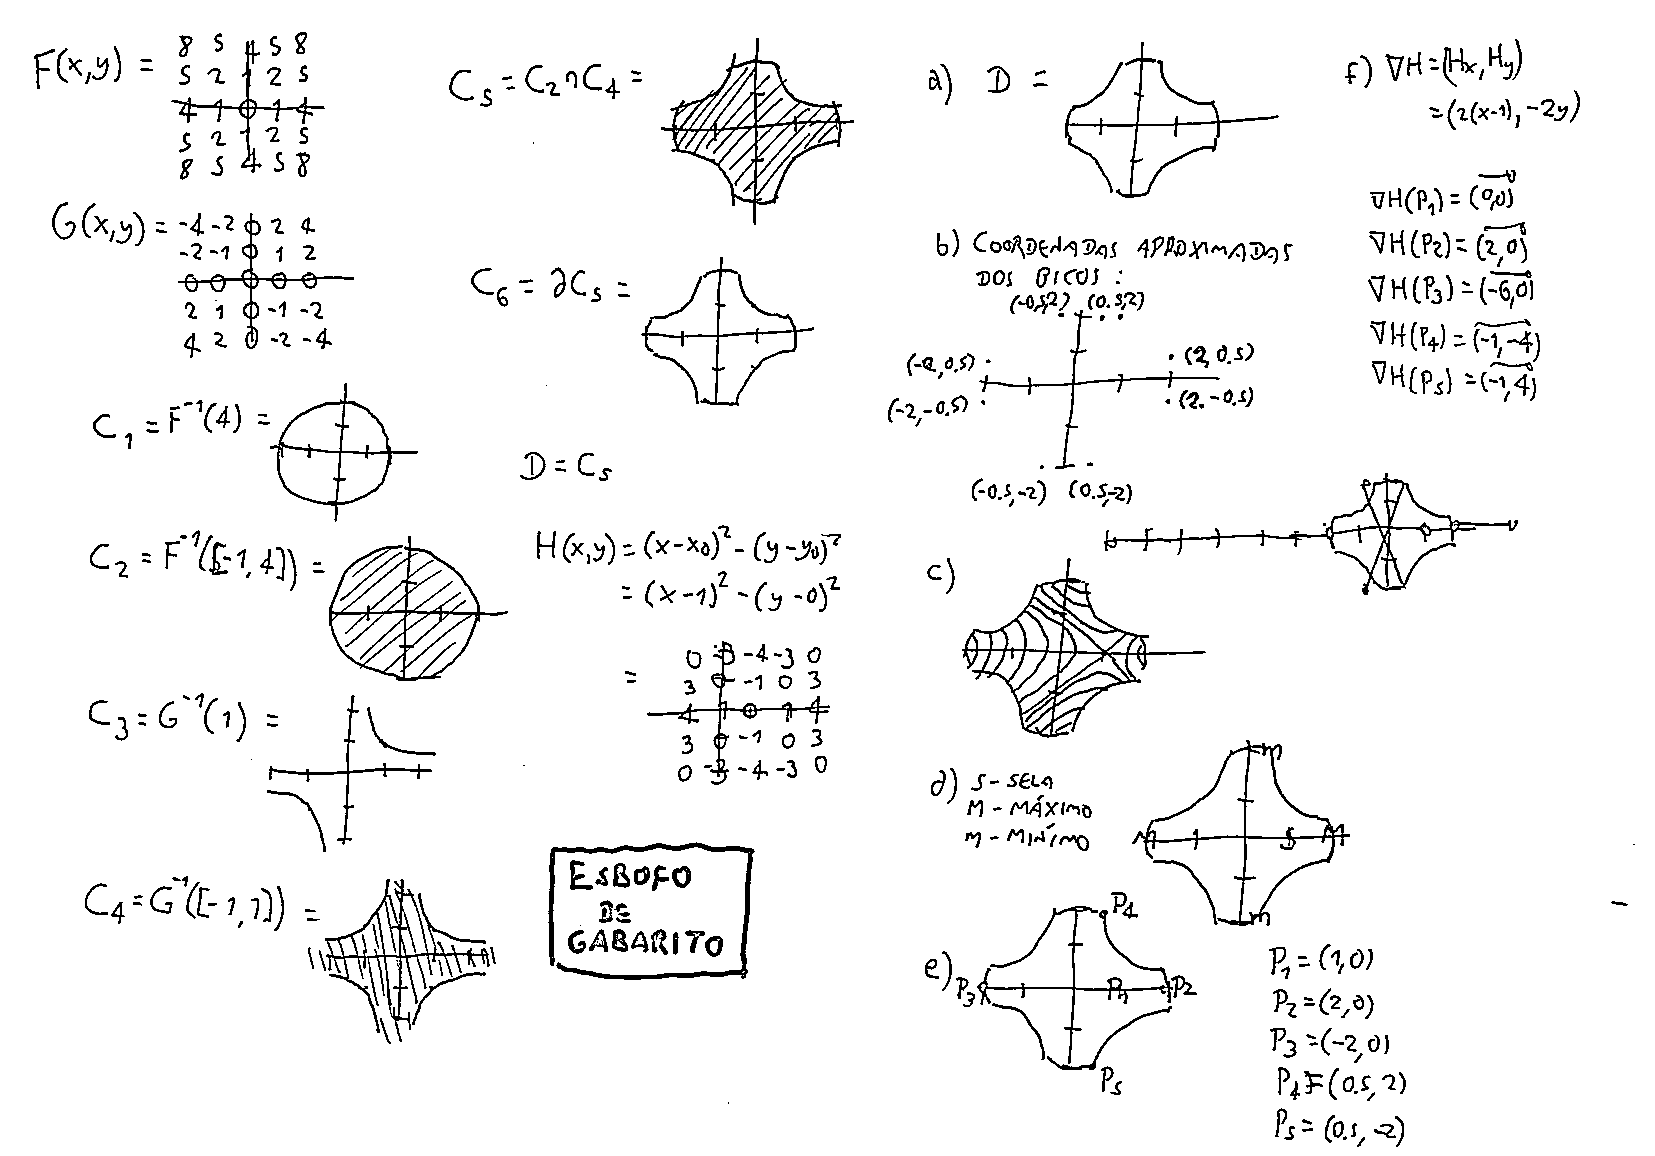
\includegraphics[height=8cm]{2022-2-C3/C3-VR-Esboco_de_gabarito.pdf}



\GenericWarning{Success:}{Success!!!}  % Used by `M-x cv'

\end{document}



 (eepitch-maxima)
 (eepitch-kill)
 (eepitch-maxima)
f2(x) := - sqrt(x^2 + 2*C3);
diff(f2(x), x);

estrela : dydx = -x / y;
subst([dydx=diff(f2(x),x), y=f2(x)], estrela);






 (eepitch-maxima)
 (eepitch-kill)
 (eepitch-maxima)
 (find-es "maxima" "2022-2-C3-P2-Q4")
F1(x,y)          := (x-1) * (y-1);
F1(x,y)          := (x-1) * (y-0);
F1(x,y)          := (x-1)^2 - (y-0)^2;
F0(x,y)          := x * y;
G(x,y)           := x^2 -   y^2;
H(x,y)           := x^2 + 4*y^2;

[minx,miny,maxx,maxy] : [-4,-4,4,4];
[minx,miny,maxx,maxy] : [-2,-2,2,2];
clevel (clr, eq)    := [color=clr, implicit(eq, x,minx,maxx, y,miny,maxy)];
clevels(clr, F, zs) := map(lambda([z], clevel(clr, F=z)), zs);
clevels : append(clevels(black, x*y, [1,-1]),
                 clevels(black, x^2+y^2, [4]),
                 clevels(red,    (x-1)^2-y^2, [0,1,2,3,4,5,6,7]),
                 clevels(violet, (x-1)^2-y^2, [-4,-3,-2,-1,0])
                );
draw2d(clevels);

clevels : [clevel(black, F0(x,y)=1),
           clevel(black, F0(x,y)=-1),
           clevel(red, F1(x,y)=-2),
           clevel(red, F1(x,y)=-1.5),
           clevel(red, F1(x,y)=-1),
           clevel(red, F1(x,y)=-0.5),
           clevel(red, F1(x,y)=0),
           clevel(red, F1(x,y)=0.5),
           clevel(red, F1(x,y)=1),
           clevel(red, F1(x,y)=1.5),
           clevel(red, F1(x,y)=2),
           clevel(red, F1(x,y)=2.5),
           clevel(red, F1(x,y)=3),
           clevel(black, x^2+y^2=4)
          ];
draw2d(clevels);

clevels(red, x^2, [0,1,2,3]);
append([1,2], [3,4]);

clevels : [clevel(red, F(x,y)=1),
           clevel(red, F(x,y)=2),
           clevel(red, F(x,y)=3),
           clevel(red, F(x,y)=4),
           clevel(green, G(x,y)=1),
           clevel(violet, H(x,y)=1)
          ];
           

clevels        :  [Eclevel(black, 16),
                   Hclevel(red,   -4),
                   Hclevel(orange,-3),
                   Hclevel(green,  0),
                   Hclevel(blue,   3),
                   Hclevel(violet, 4)
                  ];
draw2d(clevels);

Hlevel(z)      := implicit(H(x,y)=z, x,-4,4, y,-4,4);
Elevel(z)      := implicit(E(x,y)=z, x,-4,4, y,-4,4);
Hclevel(clr,z) := [color=clr, Hlevel(z)];
Eclevel(clr,z) := [color=clr, Elevel(z)];





%  ____  _             _         
% |  _ \(_)_   ___   _(_)_______ 
% | | | | \ \ / / | | | |_  / _ \
% | |_| | |\ V /| |_| | |/ /  __/
% |____// | \_/  \__,_|_/___\___|
%     |__/                       
%
% «djvuize»  (to ".djvuize")
% (find-LATEXgrep "grep --color -nH --null -e djvuize 2020-1*.tex")

 (eepitch-shell)
 (eepitch-kill)
 (eepitch-shell)
# (find-fline "~/2022.2-C3/")
# (find-fline "~/LATEX/2022-2-C3/")
# (find-fline "~/bin/djvuize")

cd /tmp/
for i in *.jpg; do echo f $(basename $i .jpg); done

f () { rm -v $1.pdf;  textcleaner -f 50 -o  5 $1.jpg $1.png; djvuize $1.pdf; xpdf $1.pdf }
f () { rm -v $1.pdf;  textcleaner -f 50 -o 10 $1.jpg $1.png; djvuize $1.pdf; xpdf $1.pdf }
f () { rm -v $1.pdf;  textcleaner -f 50 -o 20 $1.jpg $1.png; djvuize $1.pdf; xpdf $1.pdf }

f () { rm -fv $1.png $1.pdf; djvuize $1.pdf }
f () { rm -fv $1.png $1.pdf; djvuize WHITEBOARDOPTS="-m 1.0 -f 15" $1.pdf; xpdf $1.pdf }
f () { rm -fv $1.png $1.pdf; djvuize WHITEBOARDOPTS="-m 1.0 -f 30" $1.pdf; xpdf $1.pdf }
f () { rm -fv $1.png $1.pdf; djvuize WHITEBOARDOPTS="-m 1.0 -f 45" $1.pdf; xpdf $1.pdf }
f () { rm -fv $1.png $1.pdf; djvuize WHITEBOARDOPTS="-m 0.5" $1.pdf; xpdf $1.pdf }
f () { rm -fv $1.png $1.pdf; djvuize WHITEBOARDOPTS="-m 0.25" $1.pdf; xpdf $1.pdf }
f () { cp -fv $1.png $1.pdf       ~/2022.2-C3/
       cp -fv        $1.pdf ~/LATEX/2022-2-C3/
       cat <<%%%
% (find-latexscan-links "C3" "$1")
%%%
}

f 20201213_area_em_funcao_de_theta
f 20201213_area_em_funcao_de_x
f 20201213_area_fatias_pizza



%  __  __       _        
% |  \/  | __ _| | _____ 
% | |\/| |/ _` | |/ / _ \
% | |  | | (_| |   <  __/
% |_|  |_|\__,_|_|\_\___|
%                        
% <make>

 (eepitch-shell)
 (eepitch-kill)
 (eepitch-shell)
# (find-LATEXfile "2019planar-has-1.mk")
make -f 2019.mk STEM=2022-2-C3-VR veryclean
make -f 2019.mk STEM=2022-2-C3-VR pdf

% Local Variables:
% coding: utf-8-unix
% ee-tla: "c3vr"
% ee-tla: "c3m222vr"
% End:
